\chapter{Program Comprehension}
\label{c:Background}
Program comprehension is the activity of gaining knowledge about a software system.
On the one hand, it is a fundamental element of software engineering.
For instance, many maintenance tasks such as bug fixing, feature enhancement, refactoring, or documentation cannot be performed without having a sufficient understanding of the system at hand.

On the other hand, program comprehension constitutes a tedious activity with complex cognitive demands, and it reportedly accounts for up to 60\% of the software engineering effort \cite{corbi_program_1989, basili_evolving_1997}.
This implies that most of the time is spent on building a satisfactory understanding rather than on productive tasks.
Consequently, it comes as no surprise that program comprehension in general and particularly the question how its share of the software engineering effort can be reduced have emerged as interest areas in the software engineering field.

Section \ref{s:BackgroundComprehension} gives an overview of the research on object-oriented program comprehension.
The reasons that make it such a time-consuming task are depicted and related to the corresponding mental processes.
Section \ref{s:BackgroundAnalysis} shows why dynamic analysis is an inevitable instrument when it comes to assisting in the comprehension of object-oriented programs.
Furthermore, it depicts the problems that have hindered its broad application for a long time, and describes how Perscheid et al. propose to solve some of those problems. 

\section[Cognitive Aspects of Program Comprehension]{Cognitive Aspects of Program Comprehension%
\sectionmark{Cognitive Aspects}}
\sectionmark{Cognitive Aspects}
\label{s:BackgroundComprehension}
As depicted above, program comprehension is a tedious and time-consuming activity.
The reasons therefore are depicted in Section \ref{ss:BackgroundComprehensionDifficulties}.
Section \ref{ss:BackgroundComprehensionMentalModel} summarizes research about the mental aspects of program comprehension.
Finally, Section \ref{ss:BackgroundComprehensionMentalMap} draws conclusions about the properties that tools that are supposed to assist developers in program comprehension should exhibit. 

\subsection{Why Program Comprehension is Hard}
\label{ss:BackgroundComprehensionDifficulties}
Generally speaking, program comprehension requires to bridge the gaps between different conceptual areas.
Rugaber has identified five gaps that are particularly relevant in this context \cite{kent_program_1996}.

First, there is a gap between the application domain and the domain of programming languages.
A problem exists in the first domain, but the solution to this problem is implemented with programming languages that usually are not tailored to the application domain.
Consequently, an important task for programmers during program comprehension is to map the concepts of the application domain to the concepts in the source code.
And although this task requires knowledge from both domains, tools that are supposed to assist in program comprehension usually do not address the application domain.

The second gap is identified between the low-level functional principles of physical machines, the abstraction levels of programming languages, and the high-level design descriptions.
On the physical machine level, computer programs are nothing more than millions of bytes represented by the presence or absence of current.
As opposed to this, the abstraction level of design descriptions for instance is characterized by the description of objects and their interactions.
As a result, a further difficult task during program comprehension is the selection of relevant details on the low abstraction levels, and, the building of abstract representations on that basis.

Rugaber describes the third gap as discrepancy between coherent models and incoherent artifacts.
At the design time of a program and the initial implementation of a design, programs are coherently structured.
However, by the time program comprehension is required, the high-level design documents might have gotten out of date or might even be lost.
Furthermore, the original structure of the program might be completely altered through maintenance activities like feature enhancement or bug fixing.
Consequently, developers have to understand the high level architecture of a program whose original purpose may have been shifted massively.

The fourth gap lies between the formal world of computer programs and the associative nature of human cognition.
Programs are subject to strict syntactic and semantic rules that on the one hand control how they are executed but on the other hand limit how ideas can be expressed.
In contrast, human cognition is said to work associatively.
That means that patterns are detected within raw data, and relations between detected patterns are built subsequently.
In the context of program comprehension, this means that developers have to find patterns in the application domain, in their knowledge of the programming language and related best practices, as well as in data structures and algorithms.
Only if correct relations between those patterns can be built, a program will be understood.

According to Rugaber, the fifth and last discrepancy gapes between program analysis and model synthesis.
Program analysis is a bottom-up activity.
Developers try to detect low level patterns that reveal some intent, and subsequently identify the purpose of higher-level constructs these patterns are part of.
As opposed to this, model synthesis is a top-down activity.
Developers have an overall idea of the purpose of a program, and this idea is refined successively through the consideration of lower-level details.
During the process of program comprehension, both of these activities have to be accomplished at the same time.

\subsection{The Mental Model Approach to Program Comprehension}
\label{ss:BackgroundComprehensionMentalModel}
Many different models have been proposed that aim at describing the process of program comprehension.
Hierarchical plan models as proposed by Shneiderman \cite{shneiderman_exploratory_1976} or by Soloway and Ehrlich \cite{soloway_empirical_1984}, and programming strategy models as proposed by Davies \cite{davies_role_1991} are popular representatives.
However, the approach that emerged as the dominant one is the mental model approach.
Mental models describe the current state of understanding of the system under observation, and are successively updated during the process of comprehension.
They are not to be confused with cognitive models, which describe how information is processed and how this contributes to the construction of a mental model.

The mental model approach originally has been established in the context of text comprehension, for instance by van Dijk and Kintsch \cite{van_dijk_strategies_1983}, and has been adapted to procedural program comprehension by Pennington \cite{pennington_comprehension_1987, pennington_stimulus_1987}.
With the help of empirical studies, she verified the existence of two different mental representations which are built during program comprehension.
First, the program model represents the textual representation of a program as well as information about control flow and elementary operations.
Experiments have shown that this model typically emerges first, since participants tended to follow a bottom-up comprehension strategy.
Second, the domain model represents entities from the application domain and their relationships.
According to Pennington, function and data flow information also are to be attributed to this model.
Analogous to the observations about the program model, the domain model typically emerged later with successive analysis of a program.

Burkhardt et al. in turn have adapted Pennington's approach to the comprehension of object-oriented programs \cite{burkhardt_mental_1997}.
They extended the domain model by what they call static and dynamic aspects.
Among others, such static aspects are information about objects, about their relationships, and about reified objects that are not part of the problem domain.
The dynamic aspects of the domain model cover communication at coarse and fine  granularity levels, or respectively communication between objects and variables.
The former can be interpreted as client-server relationships between objects, whereas the latter rather represent data flow relationships on a procedural level.
With the help of an empirical evaluation, they verified the validity of their model, and also showed that Pennington's dual model also applies to the comprehension of object-oriented programs.

\subsection{Towards a Mental Map of Objects}
\label{ss:BackgroundComprehensionMentalMap}
As depicted in the previous section, research in the area of object-oriented program comprehension unsurprisingly suggests that objects and their interactions constitute an essential part of mental models.
At the same time, as stated in Section \ref{ss:BackgroundComprehensionDifficulties}, one of the main difficulties during program comprehension is attributable to the gap between the low abstraction levels of computers and the high abstraction levels of programming languages and design documents.
This would suggest that tools that aim at assisting in program comprehension actually provide an information presentation that covers objects and their interactions.
Without doubt, it is reasonable to presume that such an information presentation could help to close this gap.

However, the opposite can be observed when looking at established development tools.
Traditional dynamic debuggers that are included in every modern IDE are exemplary for this phenomenon.
Even when being used for the debugging of object-oriented programs, the information presentation of those debuggers is centered around the call stack.
This representation shows a sequence of function calls, but objects are no first-class entities.
Consequently, questions like which objects are actually involved in the current computation and how these objects are related are typically hard to answer.
The mere fact that these debuggers could just as well be used for the debugging of procedural programs illustrates how little they are adapted to the domain of object-oriented programming.

Consequently, the information presentations as offered by debuggers and other widely used development tools hardly seem to be suitable to aid in the construction of a mental map of objects.
This disparity raises the question why tools that offer information at the abstraction level of objects and their interactions have not been established successfully to the present day.
A major reason might be that the analysis of object interactions necessarily implies the application of dynamic analysis techniques, which struggle from major problems themselves.
A detailed insight into the necessity of dynamic analysis in this context, its problems, and a possible solution is presented in the following section.

\section{Dynamic Analysis: A Necessary Evil}
\label{s:BackgroundAnalysis}
When it comes to the analysis of objects and their interactions, the application of dynamic analysis techniques is inevitable.
The reasons for this necessity are depicted in Section \ref{ss:BackgroundAnalysisNeccessity}.
However, dynamic analysis suffers from four major problems that have prevented its broad adaption for a long time.
These problems are illustrated in Section \ref{ss:BackgroundAnalysisProblems}.
Finally, Section \ref{ss:BackgroundTracing} shows how Perscheid et al. propose to solve some of these major problems.

\subsection{The Need for Dynamic Analysis}
\label{ss:BackgroundAnalysisNeccessity}
Program comprehension usually is facilitated through two different analysis techniques, namely static and dynamic analysis.
Static analysis is executed solely with the help of source code entities.
Common examples of information that can be derived via such analyses are inheritance relationships and metrics like cyclomatic complexity or lines of code.
Furthermore, lint-tools and static code verifiers fall within the same category.
Static program analysis has two advantages.
First, it is complete in the sense that all of the source code can be considered, and the derived information holds true for all executions of a program.
Second, many static analyses can be performed rapidly.
However, this factor is largely dependent on the deepness of the analysis, and especially in the case of formal verification tools runtime is an issue \cite{wichmann_industrial_1995}.

However, when it comes to the analysis of objects and their interactions, information is required that no longer can be derived from the source code alone.
Due to object oriented concepts like polymorphism and late binding, the concrete manifestation of static source code entities is only known at runtime.
Object-oriented code defines classes and their relationships rather than collaborations of objects, which are spread throughout the code.
Furthermore, polymorphism can hide which classes actually get instantiated at runtime.
The consequence is a huge gap between the structure of the source code, and the runtime structure of programs that consists of a network of collaborating objects.
Gamma et al. use the following analogy to describe this disparity:

\begin{quote}
Trying to understand one from the other is like trying to understand the dynamism of living ecosystems from the static taxonomy of plants and animals, and vice-versa.
\par\raggedleft--- \textup{Gamma et al.}, \cite{gamma_design_1995}
\end{quote}

Consequently, it is inevitable to investigate the properties of a running system in order to draw conclusions about objects and their interactions.
This procedure is known as dynamic analysis \cite{bell_concept_1999}.

Dynamic analysis has the advantage that it is goal-oriented, meaning that specific scenarios can be executed and analyzed that cover the functionality the developer is interested in.
Furthermore, it is precise in the sense that polymorphic method calls and late binding can be resolved.
However, this comes at the cost of completeness, since dynamic analysis never can cover any possible behavior of a software system, but only that displayed during the analyzed execution.

In summary, in can be stated that there is no way around the application of dynamic analysis techniques when it comes to the exploration of objects and their interactions.
However, dynamic analysis entails severe problems that hindered its broad application for a long time.

\subsection{The Four Problems of Dynamic Analysis}
\label{ss:BackgroundAnalysisProblems}
Conventional dynamic analysis suffers from four closely related problems.
Primarily, it has a negative impact on the time that has to be spent on program comprehension, since developers have to wait long for the results of an analysis.
Furthermore, the amount of data that arises during program analysis poses a problem. 
It is difficult to store and to process, and once processing is finished, developers are confronted with much more information than they are capable of perceiving.

\subsubsection{Execution Time}
In order to get an insight into the behavior of a software system at runtime, the execution of said system has to be recorded somehow.
The most common approach for this purpose is instrumentation, which can be done at the source code or byte code level.
In this process, code is automatically added to the program under observation before its execution.
For instance, this could be tracing calls before and after every method execution which subsequently record the methods that get executed and their chronological order.

Another common strategy is to exploit debug interfaces to simulate the execution of a program.
For instance, the Java Virtual Machine Debug Interface (JVMDI) can be utilized to step through a program automatically.
At the same time, the internal state of the program can be inspected.
Thus, a trace of the call stack and of the effects of method executions on program state can be recorded.

Less common approaches in the field of dynamic program analysis are sampling techniques, which are usually used for performance measurements, and tracing at the level of the virtual machine.

But regardless of the strategy that is chosen, all these approaches slow down the execution of the system under observation massively.
Instrumented program executions are reported to be 15 up to over 100 times slower compared to undisturbed executions \cite{pothier_scalable_2007, karran_synctrace:_2013}.
For instance, Karran reports that the instrumented execution of the Firefox browser and the subsequent loading of a Google search result page take up to two minutes \cite{karran_extraction_2013}.

As a consequence, developers have to wait a long time for the generation of an execution trace.
In other words, developers already have to wait before they even can start with the analysis of the behavior of a program.
Provided that dynamic analysis tools are actually used by developers, this idle time then directly plays a part in contributing to the amount of time that is spent on program comprehension.

\subsubsection{Trace Size}
At the time of a tracing execution it is not yet known which information will actually be required during analysis.
Consequently, conventional dynamic analysis tools collect the entirety of information that might be relevant to the developer up front.
On the one hand, that means that many datasets are created which later do not matter to the developer.
On the other hand, much of the information has to be omitted during tracing, since otherwise the amount of data that has to be stored would get out of hand.
For instance, arguments of method invocations or the temporal progress of object state changes are rarely covered by traditional tracing tools (cf. Section \ref{s:RelatedTraceVis}).

As a result, the traces that result from dynamic analysis become very large, even though most tools only cover the sequence of method invocations.
For instance, Karran et al. report that the start-up of the Firefox browser alone yields 1GB of trace data \cite{karran_extraction_2013}.
Pothier et al. state that a tracing session of the Eclipse IDE that involved the creation of classes, editing of source code, and a step-by-step execution with the debugger resulted in a trace file of 33GB \cite{pothier_scalable_2007}.

This issue is so prevalent that tackling it has become a research area of its own, and diverse suggestions have been made.
For instance, Pothier et al. propose to distribute traces across different machines to allow for efficient querying and storage \cite{pothier_scalable_2007}.
Other authors suggest the application of pattern recognition strategies in order to  replace recurring patterns with representative occurrences \cite{de_pauw_execution_1998, systa_shimba_2001, richner_using_2002}.
And still others propose specialized file formats that are supposed to reduce the disk space that is consumed by execution traces \cite{johnson_lossless_1994, milenkovic_exploiting_2003}.
However, none of these proposals constitutes a fundamental change to the way of doing dynamic analysis.

\subsubsection{Processing Time}
The factor of processing time is closely related to the size of execution traces.
The larger a trace becomes, the longer it takes to process the amount of data and consequently also to present results to developers.
Measurements of this overhead rarely can be found in literature.
However, the fact that Pothier et al. identified the necessity to distribute the analysis of execution traces across multiple machines illustrates the gravity of this issue \cite{pothier_scalable_2007}.
Again, waiting time is introduced through tools that aim at assisting in program comprehension, which is equivalent to a slow-down of this process.

\subsubsection{Information Presentation and Cognitive Load}
When it comes to the presentation of trace information, one can observe a paradox situation.
On the one hand, developer tools present way too much information at the same time, and often significant amounts of this information are irrelevant in specific scenarios.
This mass of information leads to cognitive as well as informational overload.
As a consequence, developers are unable to perceive the entirety of information, and moreover, the wealth of information make it harder to draw conclusions \cite{hiltz_structuring_1985, sheridan_man-machine_1981}.

On the other hand, information that might be relevant for developers is missing, because it has not been covered during tracing.
For instance, the history of object states over the course of time is rarely covered by dynamic analysis tools (cf. Section \ref{s:RelatedTraceVis}).
This reflects the fact that the amount of information that has to be collected with up-front tracing approaches is too high.

Typically, dynamic analysis tools try to tackle this problem by providing filtering facilities either at tracing or at visualization time.
Alternative approaches automatically reduce the amount of displayed information through the application of pattern recognition techniques (cf. Section \ref{s:RelatedTraceVis}).
However, it is questionable if this strategy is sufficient to give an adequate insight into the behavior of object-oriented programs at the abstraction level of objects and their interactions.

\subsection{Step-Wise Run-Time Analysis to the Rescue?}
\label{ss:BackgroundTracing}
To overcome the technical issues of dynamic analysis, Perscheid et al. propose an approach called \emph{Step-wise Run-time Analysis} \citep{perscheid_immediacy_2010, perscheid_test-driven_2013}.
The essential idea is to utilize test cases as reproducible entry points into scenarios of expressive program behavior.
Instead of collecting huge amounts of data up front, the required information is collected successively in an iterative and interactive process that is steered by the developer.

The primary feature of this tracing approach is the distinction between shallow analysis and subsequent refinement runs.
During the shallow analysis phase, a trace of a selected test case is constructed that consists only of the bare minimum of information that is required for the reconstruction of the test execution.
This trace is presented to the developer who then can define which additional information is relevant for this specific scenario.
Refinements runs are performed to gather that additional information.
Thus, an extensive up-front collection of potentially useful information can be avoided.

\begin{figure}[tb]
	\centering
	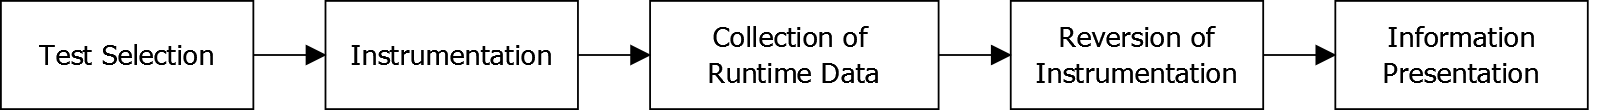
\includegraphics[width=0.9\textwidth]{../images/02-TracingProcess}
	\caption[TOC Caption]{Tracing foo}
	\label{fig:BackgroundTracingApproach}
\end{figure}

\subsubsection{Shallow Analysis}
Figure \ref{fig:BackgroundTracingApproach} depicts the fundamental steps that are performed by the \textsc{PathTools} tracing framework to generate an execution trace.
First, the user has to define a tracing scope by selecting the packages that should be considered during tracing.
Then, the user selects a test case of interest that should be traced and visualized.
For instance, this selection can be done through the list of test coverage information that is displayed next to methods in the source browser provided by the \textsc{PathTools} framework.
A \inlinecode{Tracer} object is generated which subsequently initiates the instrumentation phase.
Each method that lies within the user-defined tracing scope is replaced by a \inlinecode{MethodWrapper} that contains the fundamental tracing functionalities.

Method wrappers \cite{brant_wrappers_1998} offer a convenient way to intercept the execution of specific methods.
As the name suggests, they wrap instances of \inlinecode{CompiledMethod} and take their place in the method dictionary of the corresponding class.
They can be utilized to execute code before and after the invocation of the wrapped method.
Furthermore, they allow the inspection and manipulation of arguments as well as of the return value of a message send.
Thereby, the operation of method wrappers is fully transparent for the callers of wrapped methods.

Afterwards, the tracer executes the specified test case.
Since all methods of interest are instrumented at this stage, they automatically report their execution to the tracer.
As method entry and exit events are recorded, a call tree of the selected test case can be constructed.

Once the execution of the test case finishes, the tracer triggers the de-instrumentation phase.
The previously created method wrappers are removed from the method dictionaries and the wrapped compiled methods are put back into their original places.

\subsubsection{Refinement Runs}
Conceptually, refinement runs are very similar to the shallow analysis process.
The differences are that no test case has to be selected, since the tracer already has a reference to the covered test case.
Furthermore, only those methods are instrumented that are actually required to collect the data that should be refined.
For instance, if the developer queries the state of an argument for a specific message send, only this method is instrumented.
Afterwards, the test is executed again and the installed method wrapper verifies if the current message send is the one the developer specified.
If this is the case, the state of this argument is recorded and reported to the tracer.
Once the test execution is finished, all method wrappers are removed, and the trace visualization can be updated with the refined information.

The fundamental prerequisite of this strategy is that test cases are strictly deterministic (cf. Section \ref{ss:DiscussionLimitationsTestQuality}).
Otherwise, the returned information might not be related to the developer's query.
For instance, the state of a different object might be returned when a method is called with different arguments in repeated executions.
Additionally, non-deterministic branching that yields a diverging call tree could have the consequence that the refinement run never reaches the specified point of the execution.

\subsubsection{Information Presentation}

\begin{figure}[tb]
	\centering
	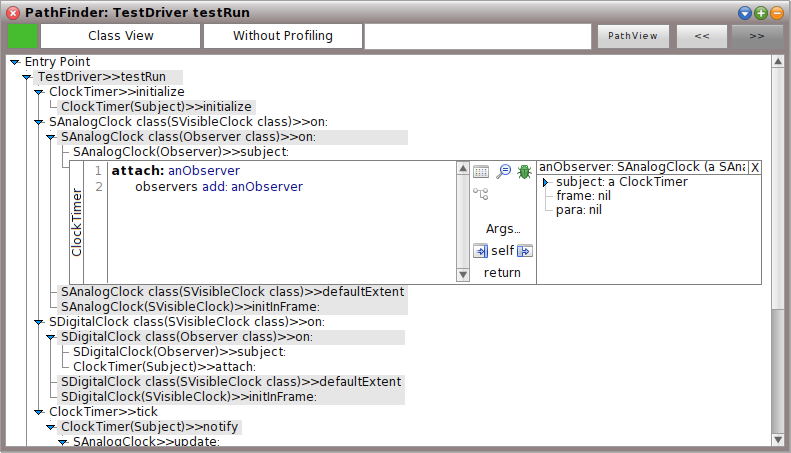
\includegraphics[width=0.9\textwidth]{../images/02-TracingPathFinder}
	\caption[Information Presentation Provided by PathFinder]{Information presentation provided by \textsc{PathFinder}, the lightweight back-in-time debugger that implements \emph{step-wise run-time analysis}.}
	\label{fig:BackgroundPathFinder}
\end{figure}

Figure \ref{fig:BackgroundPathFinder} shows the lightweight back-in-time debugger named \textsc{PathFinder} that implements the \emph{step-wise run-time analysis} approach.
As depicted, it presents a call tree of the current test execution to the developer.
Single nodes can be expanded, revealing further details like the underlying source code.
Refinement runs are performed in the background when features like state exploration are used.
Thus, developers can inspect the state of arguments, of return values, and of the receiving object before and after the execution.
Thereby, none of this information is collected up-front.

However, the provided information presentation still is rather technical.
A call tree is not a representation that conforms to the events on the abstraction level of objects.
The debugger shows a sequence of method invocations rather than objects and their interactions.
Consequently, it is still hard to figure out which objects participate in the current computation.
Furthermore, the relationships between those objects are not immediately obvious.
They have to be figured out by the developer manually, and this activity is potentially time-consuming.
For instance, a simple question like how many objects are present in an execution trace is tedious to answer with the provided instruments.

What this all amounts to is that \emph{step-wise run-time analysis} constitutes a practicable solution for three of the four major problems of dynamic analysis, namely for computation time, trace size, and processing time.
However, the presented information representation still does not play a part in closing the gap of abstraction levels.
\textsc{PathFinder} displays execution traces of object-oriented programs, but objects and their interactions are no first-class entity.
Consequently, developers still are not assisted in the creation of a mental map of objects.

%%=====================================================

\section[Modeling of Objects, States, and Interactions]{Modeling of Objects, States, and Interactions%
\sectionmark{Modeling}}
\sectionmark{Modeling}
\label{s:BackgroundModeling}
The manner in which information is presented to the observer plays an important role in human reasoning.
Accordingly, it stands to reason that the reuse of already known modeling elements in a tool that aims at aiding in the comprehension of object-oriented programs would turn out beneficial.
This raises the question which metaphors and notations already have been established in this area.

Unsurprisingly, the Unified Modeling Language, which can be regarded as the de-facto modeling standard in the field of software engineering, includes notations for object relationships and interactions.
These notations are illustrated in Section \ref{ss:BackgroundModelingUML} with the aid of an example scenario, which is depicted in Section \ref{ss:BackgroundModelingExample}.
Finally, Section \ref{ss:BackgroundModelingChallenges} discusses these diagram notations and shows potential problems and deficiencies for our area of application.


\subsection{Motivating Example}
\label{ss:BackgroundModelingExample}

\begin{figure}[tb]
	\centering
	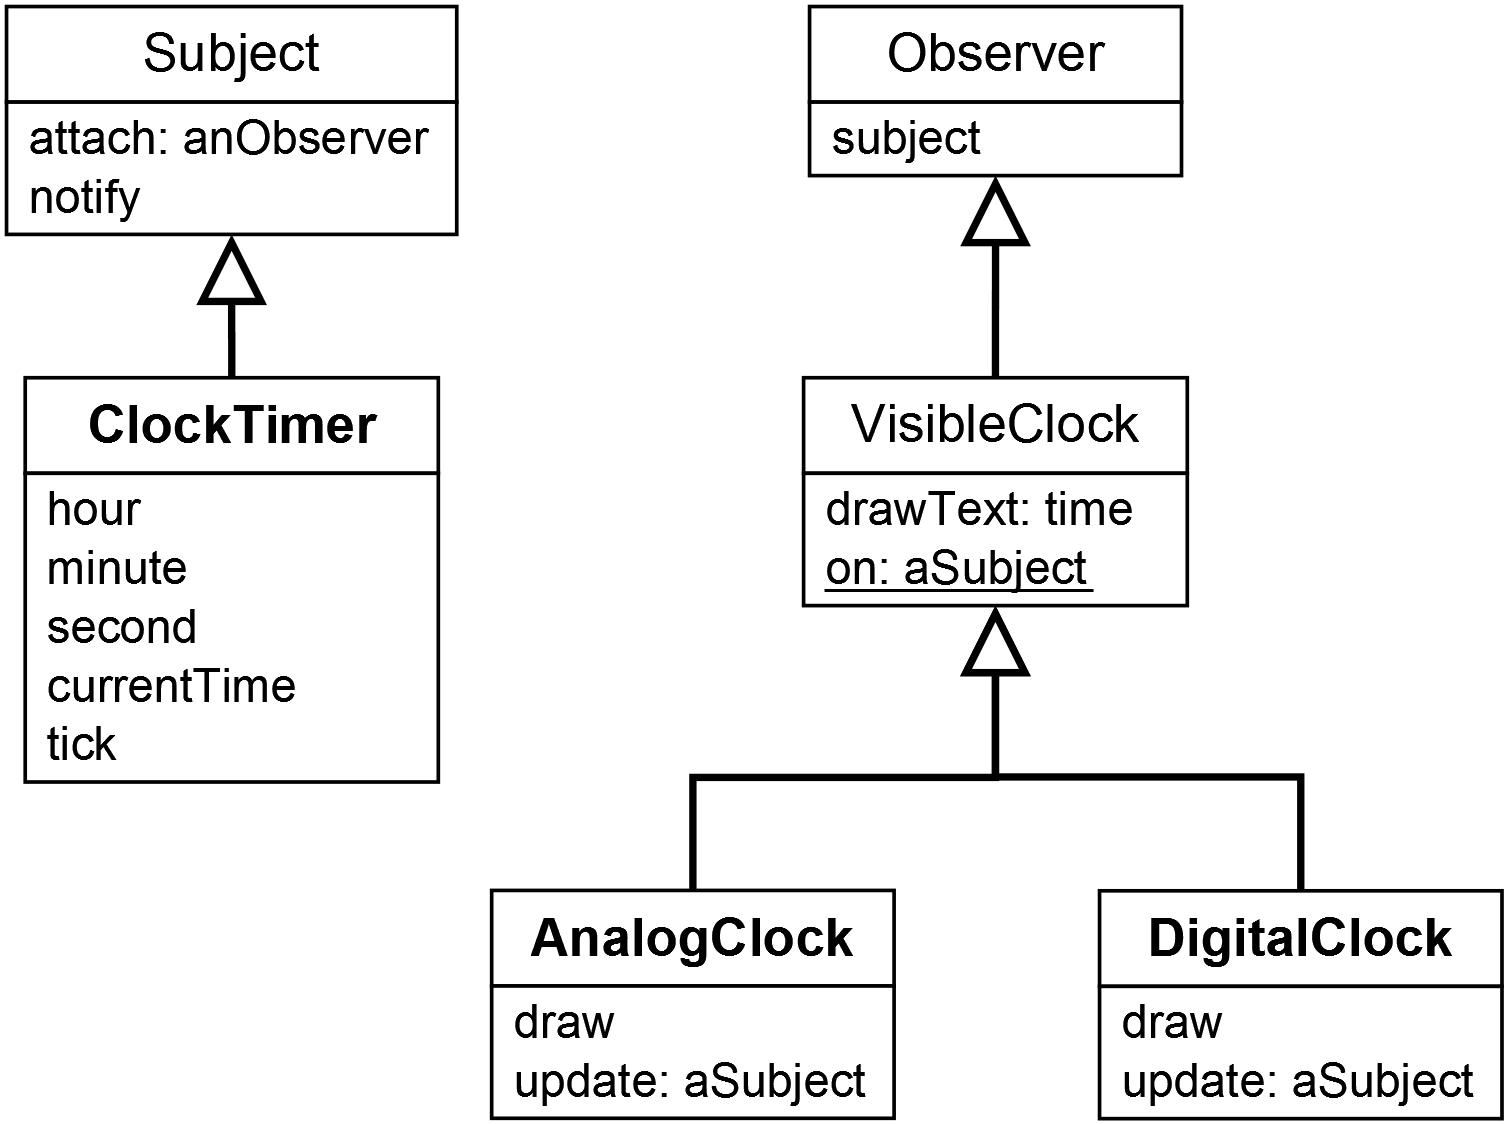
\includegraphics[width=0.7\textwidth]{../images/02-ObserverExample}
	\caption[foo]{Foo}
	\label{fig:BackgroundExample}
\end{figure}

Throughout the following chapters, the manifestation of the observer pattern \cite{gamma_design_1995} that is depicted in Figure \ref{fig:BackgroundExample} will serve as an illustrating example.
The component that emits events and thus functions as the \inlinecode{Subject} is a clock timer.
It has internal state describing the current time and provides various accessors to this state.
In addition, an interface which allows to increment the clock timer is exposed through the \inlinecode{tick} method.

Several clock visualizations can act as observers of this clock timer.
Their common base class is \inlinecode{VisibleClock}, which provides a factory method \cite{gamma_design_1995} and implements the drawing of clocks through a template method \cite{gamma_design_1995}.
\inlinecode{AnalogClock} and \inlinecode{DigitalClock} provide two different visualizations for clock timers in analog and digital fashion.
Therefore, they implement the \inlinecode{draw} method which is a part of the template method \inlinecode{drawText:}.
Furthermore, they provide an interface for subject notifications through the \inlinecode{update:} method.

The components form a pull-observer pattern, meaning that subjects notify observers of changes, but do not pass the new state along with the notification.
All observers have to pull required information from the subject on notifications.

\subsection{Objects in the Unified Modeling Language}
\label{ss:BackgroundModelingUML}
Without doubt, the Unified Modeling Language is the de-facto standard in the field of software engineering.
It is safe to assume that the majority of software developers with modeling experience have basic knowledge about it.
Consequently, it is reasonable to consider the re-use of modeling concepts, inasmuch as they are applicable to the modeling of object interactions.
Unsurprisingly, the Unified Modeling Language does indeed include diagrams that model objects and their interactions, namely object diagrams, sequence diagrams, and communication diagrams.
All three are presented in the following.

\subsubsection{Object Diagrams}

\begin{figure}
	\centering
	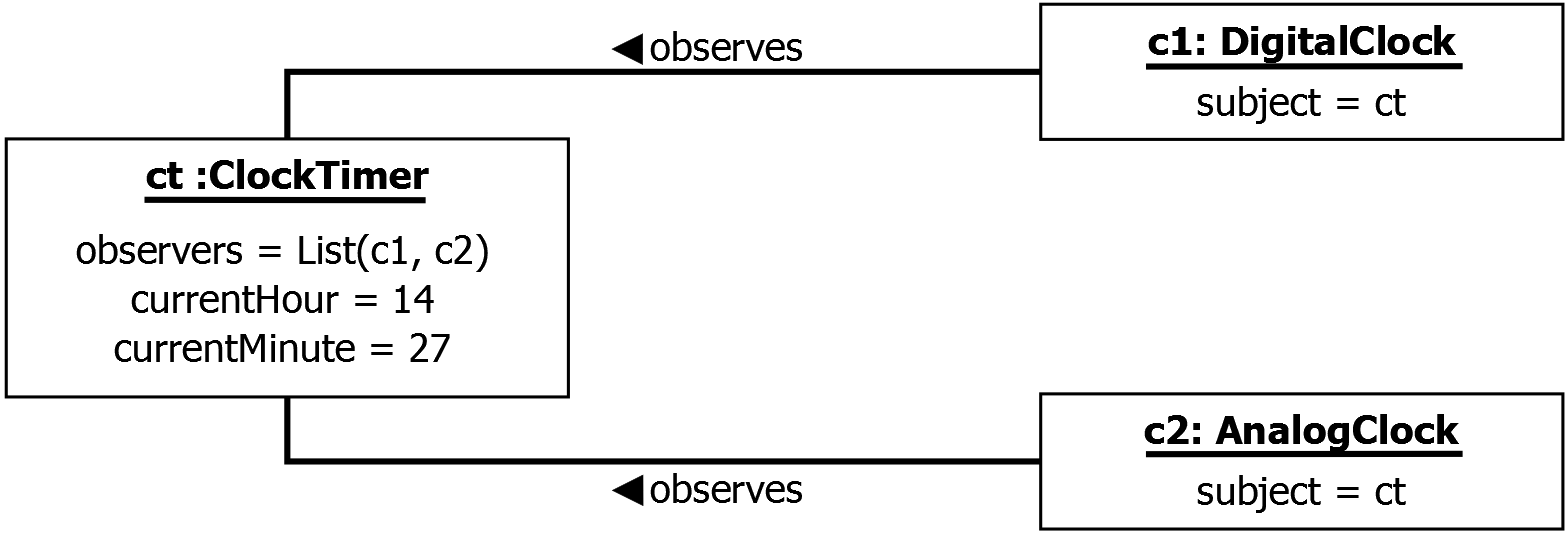
\includegraphics[width=0.7\textwidth]{../images/02-Object}
	\caption[TOC Caption]{UML Object Diagram}
	\label{fig:BackgroundModelingObject}
\end{figure}

Object diagrams \cite{rumbaugh_unified_2010} are structural diagrams that can be seen as concretization of a class diagram for a definite point in time.
As such, their notation (cf. Figure \ref{fig:BackgroundModelingObject}) covers instances and their state as well as links between instances.
The description of an instance includes an optional identifier, the type of the instance, and a list of attributes and their values.
Links can be annotated with roles and link names, whereby the latter are equipped with indicators for the reading direction.
In addition, links can be declared as forward-navigable and non-backward navigable.

Object diagrams allow the diagram creator to place objects freely on the two-dimensional canvas.
This has the advantage that objects that are closely related can be depicted in spatial proximity.
Likewise, groups of objects that are not related can be placed in different parts of the canvas.
Thus, a map of the system's runtime structure can be created that allows the observer to intuitively get an understanding of the parts of a system and their connections.

\subsubsection{Sequence Diagrams}

\begin{figure}
	\centering
	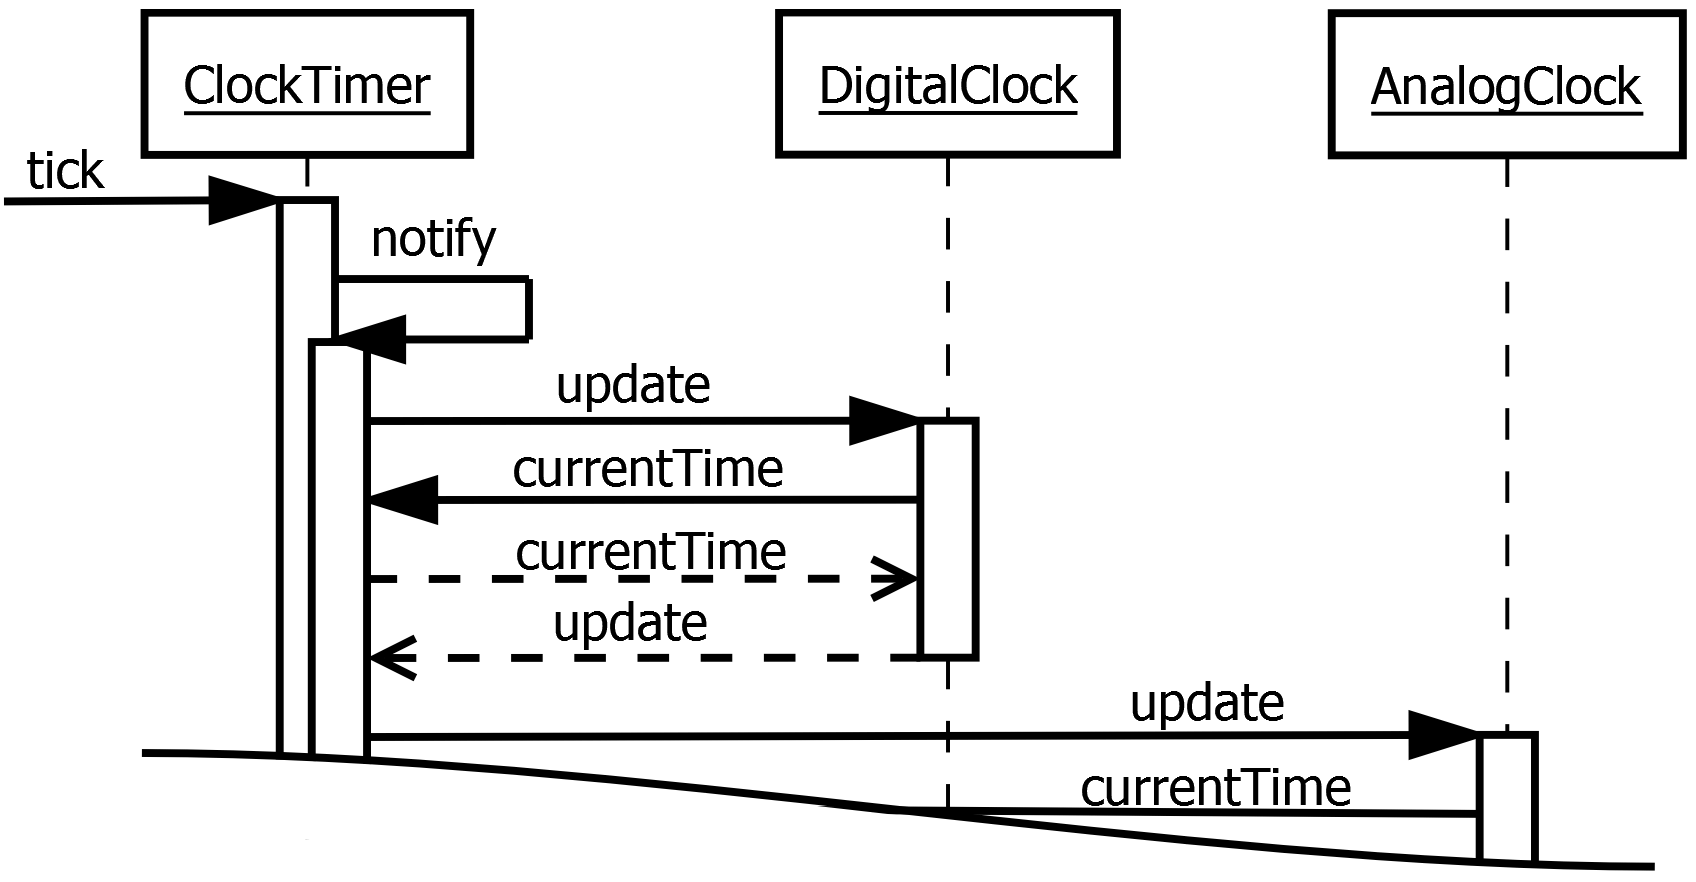
\includegraphics[width=0.6\textwidth]{../images/02-Sequence}
	\caption[TOC Caption]{UML Sequence Diagram}
	\label{fig:BackgroundModelingSequence}
\end{figure}

Sequence diagrams \cite{rumbaugh_unified_2010} are used to model the interaction of objects.
Thereby, the focus is on the exchange of messages in a specific scenario rather than the depiction of all possible execution branches.
The fundamental notation elements are depicted in Figure \ref{fig:BackgroundModelingSequence}.

Objects and their lifelines are aligned along the horizontal axis.
Execution specifications on the lifelines indicate whether an object is currently participating in a computation.
Messages between two objects are represented by arrows.
They are aligned along the vertical axis according to their chronological appearance.
Each message is complemented by a return message which indicates the end of a method invocation and which is depicted as dashed arrow.
Apart from those basic components, sequence diagrams also can be used to model duration constraints, state invariants and asynchronous behavior.
However, those advanced notation elements are of no great importance in our context.

Sequence diagrams have two major advantages.
Firstly, they feature an inherent chronological ordering, which makes following the communication thread easier for the observer.
Secondly, the automatic generation of sequence diagrams from execution traces is comparatively trivial and consequently fast, as no computation-intensive layout strategies have to be performed.
One could argue that the arrangement of the objects on the horizontal axis should be adjusted to minimize the distance between objects that exchange messages.
This optimization would certainly introduce computational complexity, but does not seem to be a common practice among the wide range of tools offering the generation of sequence diagrams that are reviewed in the related work section (cf. Chapter \ref{c:relatedwork}).

\subsubsection{Communication Diagrams}

\begin{figure}
	\centering
	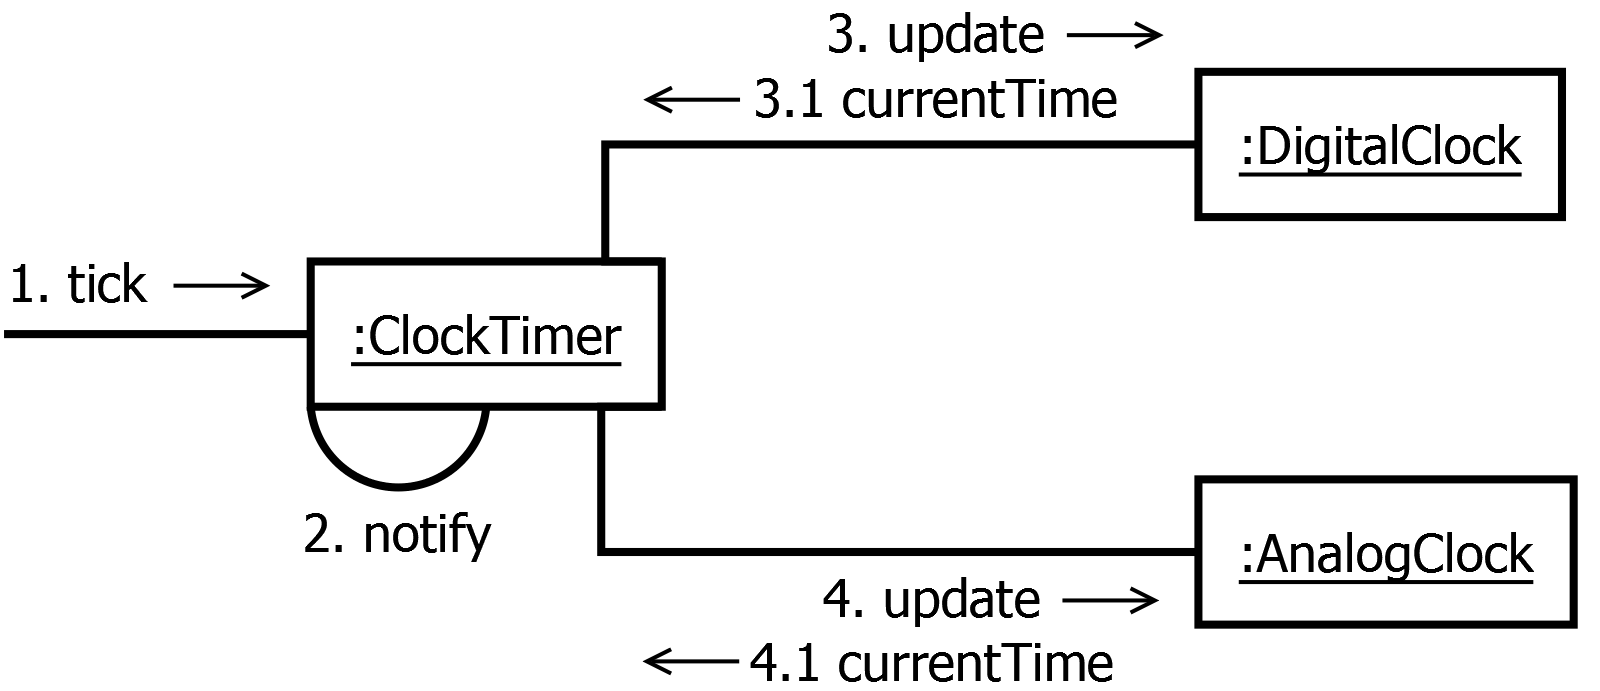
\includegraphics[width=0.6\textwidth]{../images/02-Communication}
	\caption[TOC Caption]{UML Communication Diagram}
	\label{fig:BackgroundModelingCommunication}
\end{figure}

Similar to sequence diagrams, communication diagrams \cite{rumbaugh_unified_2010} are used to model the exchange of messages between objects during a specific scenario.
However, the latter rather focus on the relationships between participating objects than on the sequence of exchanged messages.
The notation elements that are used in communication diagrams (cf. Figure \ref{fig:BackgroundModelingCommunication}) are similar to the fundamental components of sequence diagrams.
Objects are depicted as lifelines, but everything except the header is omitted.
Objects that are related through message exchanges are connected with an undirected line.
Messages between objects are aligned along those connectors and an orientation indicator shows which object is the sender and respectively the receiver of a message.
Since the notation does not offer an inherent ordering of messages, the sequence is determined through an explicit consecutive hierarchical numbering.

As with object diagrams, the main advantage of communication diagrams lies in the unrestricted placement of objects on the two-dimensional canvas.
It is for this reason that they are often used complementary with sequence diagrams, since the latter are not particularly suitable to communicate which objects belong together in consequence of their communication.

\subsection{Challenges}
\label{ss:BackgroundModelingChallenges}
Due to the fact that the Unified Modeling Language makes a strict distinction between structural and behavioral diagrams, none of them offers a combined view on object interactions as well as the internal state of objects.
However, to understand the behavior of object-oriented systems, it is important to get an insight into both.
Interactions have to be depicted in order to make the behavior of a system perceivable to the observer.
To understand why a systems behaves the way it does, the internal state of objects has to be unveiled.

Apart from this fundamental problem, the diagrams all have drawbacks of their own that make them inadequate for our objectives.

Sequence diagrams dictate to use one dimension strictly for objects (the horizontal axis) and the second dimension strictly for messages (the vertical axis).
As a result, the extent of such diagrams grows fast and does not scale well with the number of objects and messages that shall be depicted.
Adding objects inevitably leads to an extension of the x-axis, just like adding messages inevitably leads to an extension of the y-axis.
With regard to the extent requirements, it would be much more efficient to allow objects to be placed freely on the canvas, and to route messages between and around objects.
Though our objective is to depict single test cases which are comparatively small units in a software system, they usually still involve dozens of objects and messages respectively.
Scenarios of this magnitude are already sufficient to cause sequence diagrams to grow enormously.
But with the growing size of a diagram, it also becomes increasingly difficult to understand its contents and the relationships between specific components.
In this regard, sequence diagrams do not seem to be the most appropriate choice when it comes down to presenting an execution trace in a manner that is perceivable efficiently.

Communication diagrams can be used to depict a sequence of message exchanges.
However, these sequences quickly become hard to follow, since there is no inherent notion of chronology.
Developers have to search the next message with the matching number manually.
With dozens of objects and messages potentially being present in a diagram, one can imagine how tedious comprehension can become.
Furthermore, communication diagrams do not provide any means to model the internal state of objects and the effects that messages have on it.

The latter use case is partially covered by object diagrams.
However, they can only depict the state of a system at one specific point of time, and
object state changes cannot be related to message exchanges.
In fact, messages are not covered at all by this diagram type.

What this all amounts to is that the diagrams defined by the Unified Modeling Language do not suite our requirements.
An information representation that can assist developers in the comprehension of object-oriented behavior has to feature object relationships and interactions relationships as well as their impact on internal state.
Furthermore, the depiction of diagrams with the scope of test cases should be adequately economical in terms of screen space consumption.
None of the presented diagram types can satisfy these requirements.